\documentclass{beamer}

\mode<presentation> {
  \usetheme{PaloAlto}
  \usecolortheme{default}
  \usefonttheme{default}
  \setbeamertemplate{navigation symbols}{}
  \setbeamertemplate{caption}[numbered]
}

\usepackage{polski}
\usepackage[utf8x]{inputenc}
\usepackage{hyperref}
\usepackage{color}
\usepackage{alltt}
\usepackage{framed}
\usepackage{listings}
\lstset{
  basicstyle=\ttfamily\tiny,
  frame=none
}
\usepackage{pgfpages}
\pgfpagesuselayout{resize to}[physical paper width=8in, physical paper height=6in]
\setbeamertemplate{footline}[page number]

\title[GIT]{GIT - system kontroli wersji}
\author{Piotr Kowalski}
\institute{Wyższa Szkoła Informatyki Stosowanej i Zarządzania}
\date{\today}

% ------------------------------------------------------------------------------

\begin{document}
	
% --------------------------------------

\begin{frame}
  \titlepage
\end{frame}

% --------------------------------------

\section{Wprowadzenie}

\begin{frame}{Wprowadzenie}
\begin{itemize}
  \item Co to jest system kontroli wersji?
  \item Dlaczego \texttt{GIT} zdobył serca inżynierów?
\end{itemize}
\vskip 1cm
\begin{block}{System kontroli wersji}
Oprogramowanie służące do śledzenia zmian głównie w kodzie źródłowym oraz pomocy programistom w łączeniu zmian dokonanych przez wiele osób w różnych momentach.
\end{block}
\end{frame}

% --------------------------------------

\section{Rodzina systemów}

\begin{frame}{Scentralizowane}
\begin{itemize}
  \item RCS
  \item CVS
  \item Subversion
  \item GNU CSSC, klon SCCS
  \item JEDI VCS
\end{itemize}
\end{frame}

\begin{frame}{Rozproszone}
\begin{itemize}
  \item Bazaar
  \item Codeville
  \item Darcs
  \item \texttt{GIT}
  \item GNU Arch
  \item Mercurial
  \item Monotone
  \item svk
\end{itemize}
\end{frame}

\begin{frame}{Zamknięte (własnościowe) systemy kontroli wersji}
\begin{itemize}
  \item BitKeeper firmy BitMover
  \item Code Co-op firmy Reliable Software
  \item Perforce firmy Perforce Software
  \item Rational ClearCase firmy IBM
  \item Sablime firmy Lucent Technologies
  \item StarTeam firmy Borland
  \item Visual SourceSafe firmy Microsoft
  \item Visual Studio Team Foundation Server firmy Microsoft
\end{itemize}
\end{frame}

\begin{frame}{Informacje ogólne}
\begin{block}{GIT}
Rozproszony system kontroli wersji. Stworzył go Linus Torvalds jako narzędzie wspomagające rozwój jądra Linux. \texttt{GIT} stanowi wolne oprogramowanie i został opublikowany na licencji GNU GPL w wersji 2.
\end{block}
\end{frame}

\begin{frame}{Historia}
\begin{itemize}
	\item Prace nad \texttt{GIT}em rozpoczęły się po tym, jak BitKeeper, używany wtedy do rozwoju Linuksa, przestał być darmowy dla projektów o otwartym kodzie źródłowym. 
\vskip 1cm
	\item Prace nad \texttt{GIT}em rozpoczęły się 3 kwietnia 2005 roku, projekt został ogłoszony 6 kwietnia, 7 kwietnia \texttt{GIT} obsługiwał kontrolę wersji swojego własnego kodu, 18 kwietnia pierwszy raz wykonano łączenie kilku gałęzi kodu, 27 kwietnia \texttt{GIT} został przetestowany pod względem szybkości z wynikiem 6,7 łat na sekundę, a 16 czerwca Linux 2.6.12 był hostowany przez \texttt{GIT}a.
\end{itemize}
\end{frame}

\begin{frame}{Założenia}
Torvalds szukał rozproszonego systemu kontroli wersji, który mógłby być użyty zamiast BitKeepera, głównymi kryteriami wyboru były:
\begin{itemize}
	\item Wziąć przykład z CVS, czego nie robić.
	\item System powinien być rozproszony.
	\item System powinien być chroniony przed błędami w repozytorium (przypadkowymi, jak awaria twardego dysku, jak i złośliwymi, wprowadzonymi przez kogoś).
	\item System powinien być szybki.
\end{itemize}
Pierwsze dwa punkty wyeliminowały wszystko prócz Monotone'a, a czwarty punkt wyeliminował wszystko, więc Torvalds postanowił napisać własny system kontroli wersji.
\end{frame}

% --------------------------------------

\section{Składowe}

\begin{frame}{Rewizja}
Do wprowadzenia zmian w projekcie służy specjalna \textbf{operacja zatwierdzania} \textit{(ang. commit)}. Nie jest ona nigdy wykonywana przez \texttt{GIT} automatycznie. Jeśli uznamy, że bieżacy stan plików lub folderów jest istotny, należy samodzielnie wykonać operację zatwierdzania.

\vskip 0.5cm
Operację zatwierdzania możemy w pewnym uproszczeniu traktować jako zapisanie bieżącego stanu wszystkich plików i folderów 
projektu w danej chwili.

\vskip 0.5cm
Wykonanie operacji zatwierdzania powoduje zapisanie \textbf{rewizji} \textit{(ang. commit, revision)}.
\end{frame}

\begin{frame}{Rewizja - dalej}
\begin{block}{Utworzenie rewizji}
\$ git add plik.txt \\
\$ git commit -m "dodajemy plik.txt"
\begin{alltt}
[master 66601e8] dodajemy plik.txt \\ 
 1 file changed, 0 insertions(+), 0 deletions(-) \\
 create mode 100644 plik.txt
\end{alltt}
\end{block}
\end{frame}

\begin{frame}{Branch}
Gałąź \textit{(ang. branch)} jest to inna ścieżka dla rewizji.
Domyślna gałąź to branch \textbf{master}.

Branche nie są ze sobą połączone, chyba, że zostaną zmergowane.

Stworzona rewizja istnieje tylko w jednym branchu, chyba, że zrobimy cherry-picka.
\end{frame}

\begin{frame}{Branch - local}
\begin{block}{Stworzenie nowego oraz przełączenie się na niego}
\$ git checkout -b simple-feature
\begin{alltt}
Switched to a new branch 'simple-feature'
\end{alltt}
\end{block}
\begin{block}{Usunięcie brancha lokalnie}
\$ git branch -D simple-feature
\begin{alltt}
Deleted branch simple-feature (was 2b325c2).
\end{alltt}
\end{block}
\begin{block}{Wypchnięcie brancha na serwer}
\$ git push origin simple-feature
\begin{alltt}
Total 0 (delta 0), reused 0 (delta 0) \\
To git@github.com:piecioshka/test.git \\
 * [new branch]      simple-feature -> simple-feature
\end{alltt}
\end{block}
\end{frame}

\begin{frame}{Branch - remote}
\begin{block}{Wyświetlenie wszystkich gałęzi projektu (local \& remote)}
\$ git branch -la
\begin{alltt}
  master \\
* simple-feature \\
  remotes/origin/master \\
  remotes/origin/simple-feature
\end{alltt}
\end{block}
\begin{block}{Usunięcie brancha z serwera}
\$ git push origin :simple-feature
\begin{alltt}
To git@github.com:piecioshka/test.git \\
 - [deleted]         simple-feature
\end{alltt}
\end{block}
\end{frame}

\begin{frame}{Tag}
Znacznik \textit{(ang. tag)} jest to rewizja która jest specjalnie zapisana w repozytorium.
Rewizja ta zostaje oznakowana specjnalnym komentarzem, aby w przyszłości szybciej dotrzeć to odpowiedniego etapu projektu.
\vskip 0.5cm
Przykład poprawnie stworzonych znaczników:
\begin{itemize}
  \item \url{https://github.com/adobe/brackets/tags}
\end{itemize}
\end{frame}

\begin{frame}{Tag - dalej}
\begin{block}{Stworzenie nowego znacznika}
\$ git tag v1.0 -m "new feature"
\end{block}
\vskip 0.5cm
\begin{block}{Wyświetlenie wszystkich tagów projektu}
\$ git tags -l
\end{block}
\begin{block}{Wypchnięcie tagów na serwer}
\$ git push --tags
\end{block}
\end{frame}

\begin{frame}{Wyświetlanie rewizji}
\begin{block}{Wyświetlenie rewizji w sposób czytelny}
\begin{alltt}
\$ git log --graph --pretty=oneline \\
\$ gitk
\end{alltt}
\end{block}
\end{frame}

\begin{frame}{Przykład projektu}
	\begin{figure}
	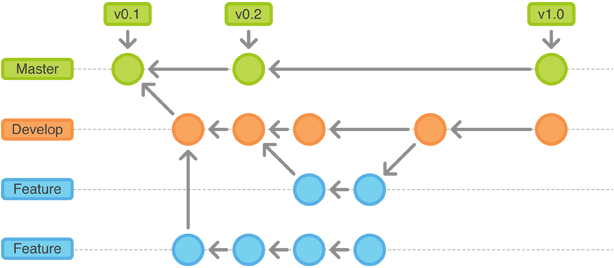
\includegraphics[width=\textwidth]{revisions_and_branches_and_tags.png}
	\caption{\label{Branches}Rewizje, branche, tagi}
	\end{figure}
\end{frame}

% --------------------------------------

\section{GIT w życiu codziennym}

\subsection{GitHub}

\begin{frame}{GitHub - rejestracja}
	\begin{figure}
	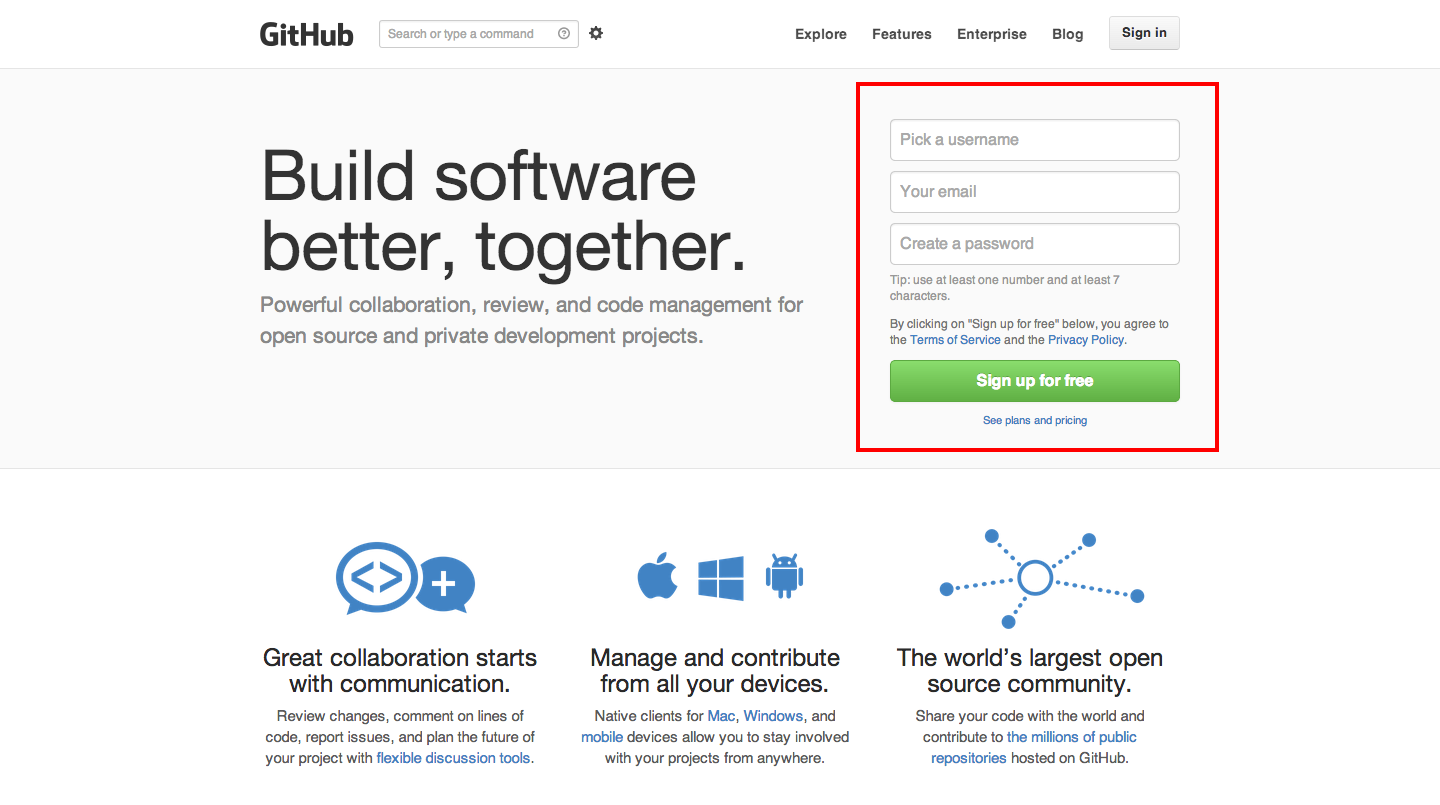
\includegraphics[width=\textwidth]{sign-up.png}
	\caption{\label{fig:sign-up}Formularz rejestracji konta}
	\end{figure}
\end{frame}

\begin{frame}{GitHub - logowanie}
	\begin{figure}
	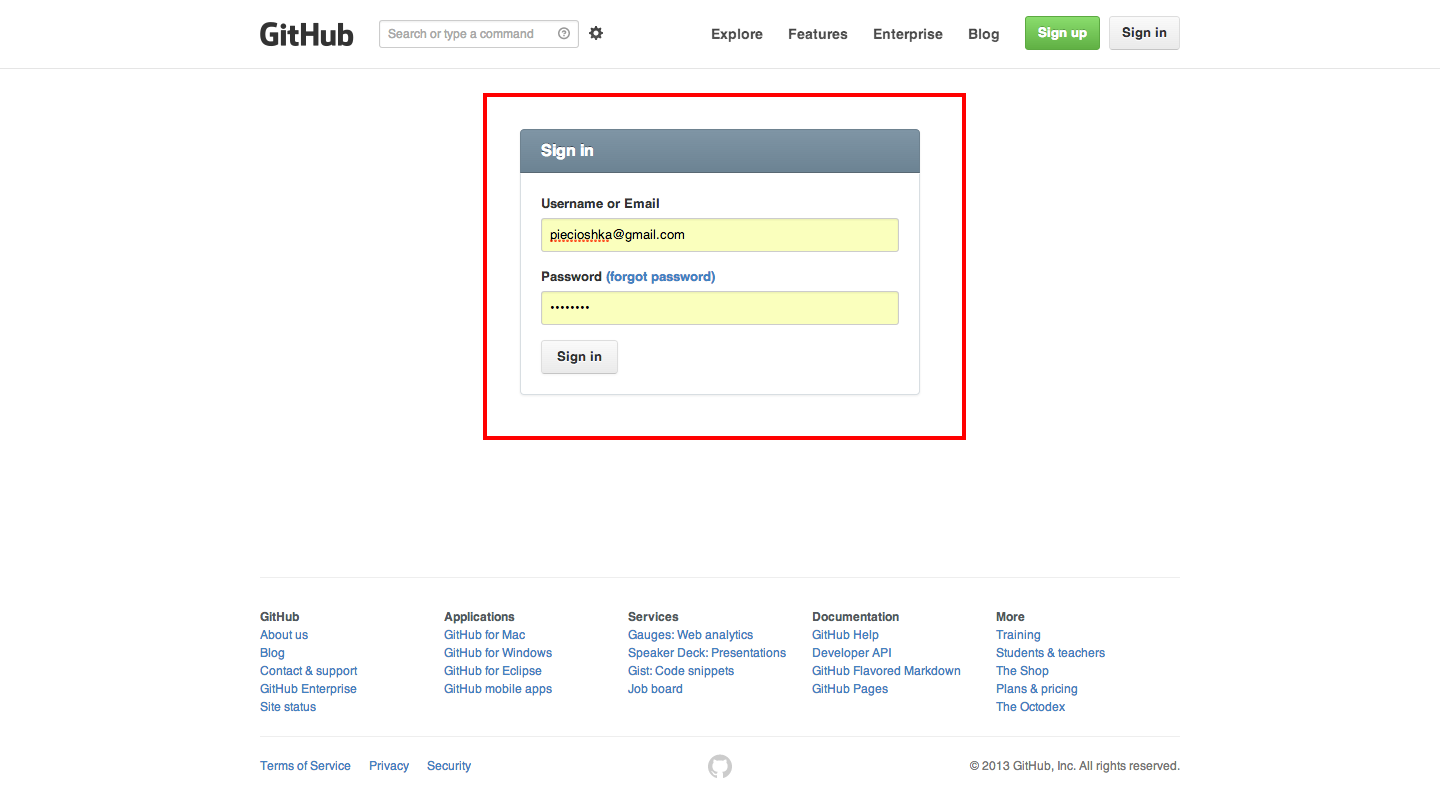
\includegraphics[width=\textwidth]{sign-in.png}
	\caption{\label{fig:sign-in}Formularz logowania użytkownika}
	\end{figure}
\end{frame}

\begin{frame}{GitHub - tworzenie nowego repozytorium}
	\begin{figure}
	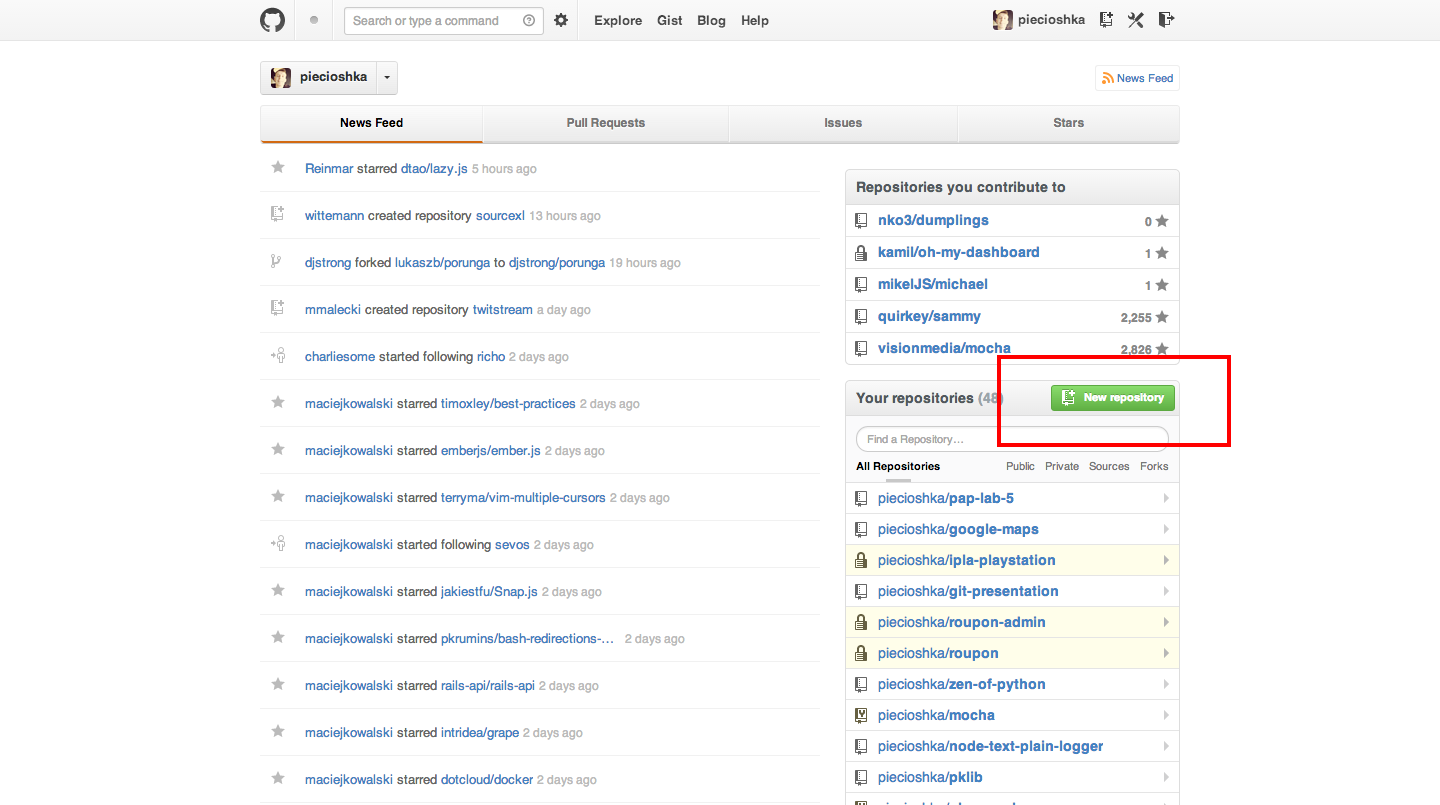
\includegraphics[width=\textwidth]{create-repo-link.png}
	\caption{\label{fig:create-repo-link}Link do utworzenia nowego repozytorium}
	\end{figure}
\end{frame}

\begin{frame}{GitHub - nowe repozytorium}
	\begin{figure}
	\includegraphics[width=\textwidth]{new-repo.png}
	\caption{\label{fig:new-repo}Ustal nazwę dla nowego repozytorium}
	\end{figure}
\end{frame}

\begin{frame}{GitHub - nowe puste repozytorium}
	\begin{figure}
	\includegraphics[width=\textwidth]{new-repo-settings.png}
	\caption{\label{fig:new-repo-settings}Początkowe ustawienia repozytorium}
	\end{figure}
\end{frame}

\begin{framed}
\begin{lstlisting}[frame=none, caption=Pierwszy projekt]
$ mkdir test && cd test
$ touch README.md
$ git init
$ git add README.md
$ git commit -m "Pierwszy commit"
$ git remote add origin git@github.com:piecioshka/test.git
$ git push -u origin master
\end{lstlisting}
\end{framed}

\begin{frame}{GitHub - projekt}
	\begin{figure}
	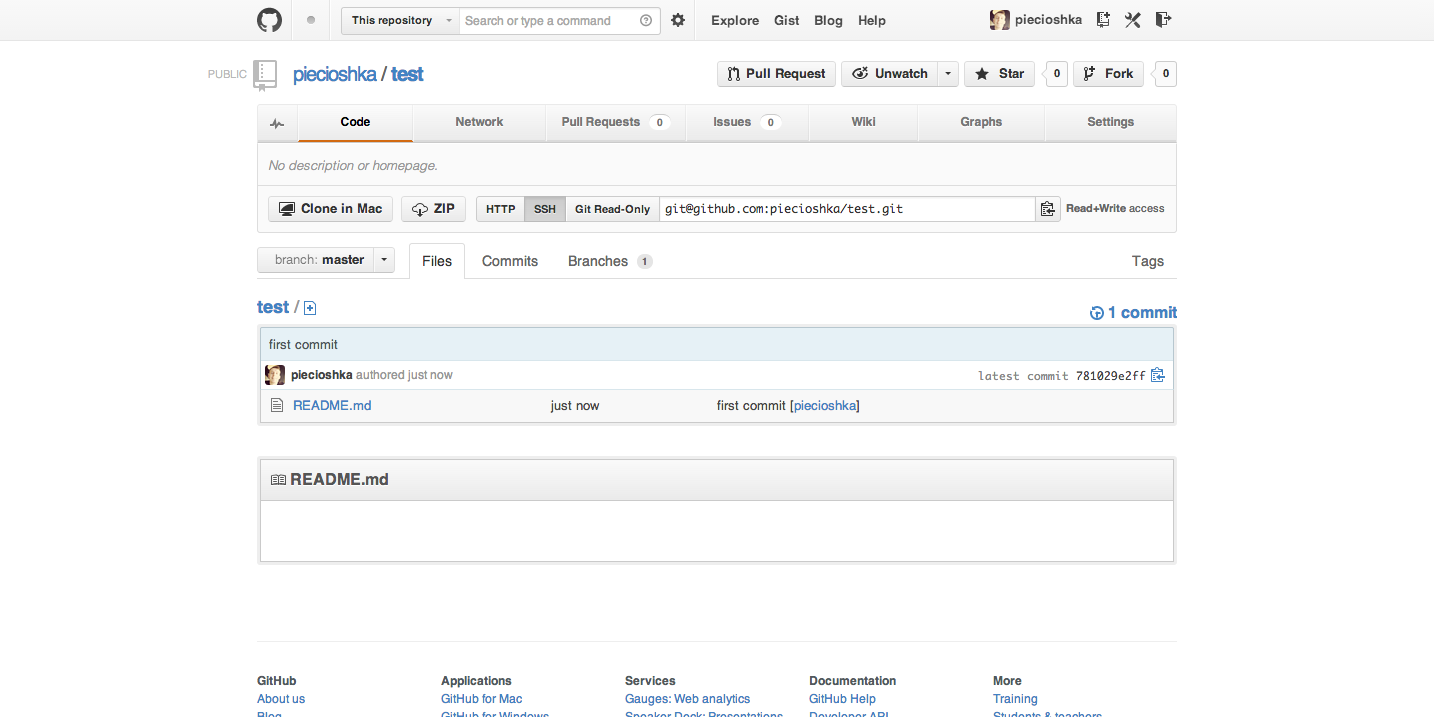
\includegraphics[width=\textwidth]{project.png}
	\caption{\label{fig:project}Projekt}
	\end{figure}
\end{frame}

\begin{framed}
\begin{lstlisting}[frame=none, caption=Praca lokalna]
$ mkdir test && cd test
$ touch README.md
$ git init
$ git add README.md
$ git commit -m "Pierwszy commit"
\end{lstlisting}
\end{framed}

\begin{framed}
\begin{lstlisting}[frame=none, caption=Praca zdalna]
$ git remote add origin git@github.com:piecioshka/test.git
$ git push -u origin master
\end{lstlisting}
\end{framed}

\begin{framed}
\begin{lstlisting}[frame=none, caption=Najpopularniejsze polecenia]
$ git add
$ git status
$ git log
$ git branch
$ git checkout
$ git diff
$ git pull
$ git push
$ git reset
$ git tag
$ git blame
$ git summary
$ git ignore
\end{lstlisting}
\end{framed}

% --------------------------------------

\section{Podsumowanie}

\begin{frame}{Podsumowanie}
\texttt{GIT} jest:
\begin{itemize}
  \item wszechstronny i uniwersalny
  \item rozproszyny
  \item przenośny
  \item multiplatformowy
  \item wygodny
  \item szybki
  \item bezpieczny
  \item darmowy
\end{itemize}
\vskip 1cm
Czego więcej potrzeba?	
\end{frame}

% --------------------------------------

\section{Wnioski}

\begin{frame}{Wnioski}
\begin{enumerate}
  \item Jak się na to zapatrujecie?
  \item Czy jest sens, używania systemu kontroli wersji, podczas działań w pojedynkę?
\end{enumerate}
\end{frame}

% --------------------------------------

\section{Linki}

\begin{frame}{Przydatne adresy WWW}
\begin{itemize}
  \item \url{http://help.github.com/}
  \item \url{http://github.com/git/git}
  \item \url{http://git-scm.com/book/pl/Pierwsze-kroki-Wprowadzenie-do-kontroli-wersji}
  \item \url{https://bitbucket.org/}
\end{itemize}
\vskip 1cm
Źródła do tej prezentacji:
\begin{itemize}
  \item \url{https://github.com/piecioshka/git-presentation}

\end{itemize}
\end{frame}

% --------------------------------------

\section{Autor}

\begin{frame}{Autor}
\begin{itemize}
  \item GitHub: piecioshka
  \item Twitter: @piecioshka
\end{itemize}
\end{frame}

\end{document}
